\chapter{Scans und Sweeps}\label{ch:scans}

\FG{} kennt zwei Arten, viele Rechnungen auf einmal zu machen:
\begin{description}
  \item[Scan] über die Einfallsparameter $\lambda$, $\varphi$, $\psi$, $\delta$. Die Scanpunkte laufen
        \emph{parallel}, die Struktur bleibt gleich.
  \item[Sweep] über eine beliebige Zahl der Konfiguration (Dicke, Breite, Brechzahl, Periode \ldots). Für jeden
        Sweep-Wert wird der ganze Scan gerechnet; die Sweep-Werte laufen \emph{nacheinander}.
\end{description}

\section{Scans}
\index{Scan}%
\subsection{Werte angeben}
\begin{lstlisting}[language=json]
"incidence": {
  "lambda_um": { "from": 0.4, "to": 0.8, "steps": 81 },   // Bereich, Endpunkte eingeschlossen
  "phi_deg":   [0, 10, 20, 30],                            // Liste
  "psi_deg":   0,                                          // Zahl
  "delta_deg": [0, 90]                                     // s und p
}
\end{lstlisting}
Gerechnet werden $81\cdot4\cdot1\cdot2=648$ Punkte, in der Reihenfolge $\lambda$ (außen), $\varphi$, $\psi$, $\delta$
(innen).

\subsection{Typische Scans}
\begin{center}
\small
\begin{tabularx}{\linewidth}{lY}
\toprule
Ziel & Einfall \\
\midrule
Spektrum, beide Polarisationen & \val{"lambda\_um": \{...\}, "delta\_deg": [0, 90]} \\
Winkelgang (Rocking Curve) & \val{"phi\_deg": \{"from": 0, "to": 80, "steps": 161\}} \\
Azimutabhängigkeit eines 2D-Gitters & \val{"psi\_deg": \{"from": 0, "to": 45, "steps": 10\}} \\
Polarisationsdrehung & \val{"delta\_deg": \{"from": 0, "to": 180, "steps": 37\}} \\
Littrow-Kurve & Python-Schleife mit $\varphi(\lambda)=\arcsin\bigl(\lambda/(2d)\bigr)$ (Abschnitt~\ref{sec:py-schleifen}) \\
\bottomrule
\end{tabularx}
\end{center}

\begin{tipp}[Unpolarisiertes Licht]
Die Effizienz für unpolarisiertes Licht ist der Mittelwert aus s und p: $e_{\text{unpol}}=\tfrac12(e_s+e_p)$.
Rechnen Sie dazu \val{"delta\_deg": [0, 90]} und mitteln Sie.
\end{tipp}

\subsection{Parallelität}
Scanpunkte laufen parallel auf allen Kernen (OpenMP). Wie viele Threads auf die Scanpunkte und wie viele auf die
Scheiben einer Rechnung entfallen, regelt \key{threads} (Abschnitt~\ref{sec:threads}). Die Ergebnisse hängen nicht
von der Threadzahl ab; sie sind bitgleich.

\section{Sweeps}
\index{Sweep}%
\subsection{Aufbau}
\begin{lstlisting}[language=json]
"sweep": {
  "parameter": "/layers/0/thickness_um",
  "values": { "from": 0.05, "to": 1.2, "steps": 24 }
}
\end{lstlisting}
\key{parameter} ist ein \textbf{JSON-Pointer} (RFC 6901) in dieselbe Konfigurationsdatei. \key{values} ist eine Zahl,
eine Liste oder ein Bereich. Für jeden Wert ersetzt \FG{} die Zahl an der Stelle des Pointers und rechnet den
gesamten Scan.

\subsection{JSON-Pointer}
Ein Pointer beschreibt den Weg durch die verschachtelte Struktur: Schlüssel von Objekten mit Namen, Listenelemente
mit ihrer Nummer ab 0, alles durch \texttt{/} getrennt.
\begin{center}
\small
\begin{tabularx}{\linewidth}{lY}
\toprule
Pointer & zeigt auf \\
\midrule
\val{/layers/0/thickness\_um} & Dicke der untersten Schicht \\
\val{/layers/1/depth\_um} & Profiltiefe der zweiten Schicht \\
\val{/layers/0/breakpoints\_um/1} & zweite Stelle einer Lamellenschicht (z.\,B.\ Stegbreite) \\
\val{/period\_um/x} & Periode in $x$ \\
\val{/materials/si/n/0} & Realteil der Brechzahl von \texttt{si} (nur wenn \key{n} als \val{[Re, Im]} angegeben ist) \\
\val{/materials/glass/n} & reelle Brechzahl von \texttt{glass} (nur wenn \key{n} eine Zahl ist) \\
\val{/layers/0/inclusions/0/rectangle\_um/size/0} & Breite eines Rechtecks in $x$ \\
\val{/layers/2/regions/0/circle/radius\_um} & Radius eines Kreises in \val{contour2d} \\
\val{/truncation/Nx} & Trunkierung (für Konvergenzstudien) \\
\val{/rcwa/slices} & Scheibenzahl (nur wenn der Block \key{rcwa} existiert) \\
\bottomrule
\end{tabularx}
\end{center}
Regeln:
\begin{itemize}
  \item Der Pointer muss auf eine \emph{vorhandene Zahl} zeigen. Andernfalls meldet \FG{}
        \texttt{sweep: parameter '...' not found} bzw.\ \texttt{is not a number}. Legen Sie optionale Blöcke deshalb
        vorher an.
  \item Ein Schrägstrich oder eine Tilde in einem Schlüssel wird als \texttt{\textasciitilde1} bzw.\
        \texttt{\textasciitilde0} geschrieben (selten nötig).
  \item Es gibt genau \emph{einen} Sweep-Parameter. Mehrdimensionale Parameterstudien rechnen Sie in Python
        (Abschnitt~\ref{sec:py-schleifen}).
\end{itemize}

\begin{achtung}[Zusammenhängende Größen]
Ein Sweep ändert genau eine Zahl. Soll die Stegbreite einer Lamelle symmetrisch um die Zellmitte wachsen, müssen sich
zwei Stellen gleichzeitig ändern -- das geht nur in Python. Ebenso gilt: Wird die Periode verändert, bleiben die
\key{breakpoints\_um} stehen. Der letzte Wert muss aber gleich der Periode sein. \FG{} prüft das derzeit
\emph{nicht}: Mit $d_x=1{,}2$ und Stellen bis 1,0 läuft die Rechnung ohne Fehlermeldung, liefert aber ein falsches
Ergebnis (erkennbar an der Energiebilanz $\neq1$ bei verlustfreien Materialien).
\end{achtung}

\subsection{Ausgabe eines Sweeps}
Die CSV-Datei erhält vorn die Spalten \texttt{sweep\_parameter} und \texttt{sweep\_value}:
\begin{lstlisting}
sweep_parameter,sweep_value,lambda_um,phi_deg,psi_deg,delta_deg,side,n,m,efficiency,...
/layers/0/thickness_um,0.05,0.6328,18.45,0,0,R,-2,0,1.36004339868e-05,...
/layers/0/thickness_um,0.05,0.6328,18.45,0,0,R,-1,0,0.00380450602064,...
\end{lstlisting}
Auf dem Terminal beginnt jeder Sweep-Wert mit einer Zeile \texttt{== sweep /layers/0/thickness\_um = 0.05}. Ein
Nahfeld wird nur für den ersten Scanpunkt des ersten Sweep-Werts berechnet.

\subsection{Beispiel: Stegtiefe einer Glaslamelle}
\file{examples/sweep\_lamellar\_depth.json} variiert die Höhe einer Glaslamelle von 0,05 bis 1,2\um{} bei
Littrow-naher Beleuchtung, für TE und TM:
\begin{lstlisting}[style=shell]
fgsolve examples/sweep_lamellar_depth.json
scripts/plot_efficiencies.py out/sweep_lamellar_depth/efficiencies.csv \
        --orders R:0 R:-1 T:0 T:-1 --delta 0 --out sweep_te.png
\end{lstlisting}
\begin{figure}[h]
\centering
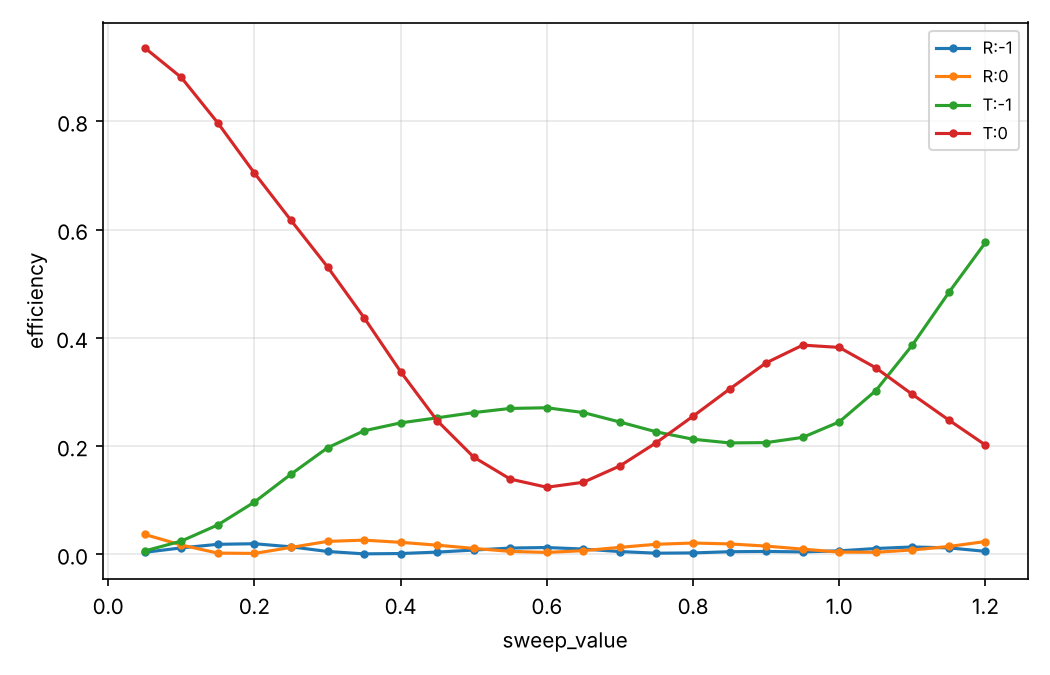
\includegraphics[width=0.78\linewidth]{fig/sweep_te.png}
\caption{Effizienzen über der Stegtiefe (TE). Die nullte Transmissionsordnung wird bei etwa 0,6\um{} Tiefe
weitgehend unterdrückt; dort geht die Leistung in die Ordnung $-1$.}
\end{figure}

\section{Darstellung mit \texttt{plot\_efficiencies.py}}
\begin{lstlisting}[style=shell]
scripts/plot_efficiencies.py CSV [--x SPALTE] [--orders R:0 T:-1 ...] [--quantity efficiency|eff_s|eff_p]
                                 [--lambda W] [--phi W] [--psi W] [--delta W] [--out bild.png]
\end{lstlisting}
\begin{itemize}
  \item Die $x$-Achse ist die erste veränderliche Spalte aus \texttt{sweep\_value}, \texttt{lambda\_um},
        \texttt{phi\_deg}, \texttt{psi\_deg}, \texttt{delta\_deg} oder die mit \texttt{-{}-x} gewählte.
  \item \texttt{-{}-orders} wählt Ordnungen als \texttt{Seite:n} oder \texttt{Seite:n:m}; ohne Angabe alle.
  \item Die übrigen veränderlichen Spalten halten Sie mit \texttt{-{}-lambda}, \texttt{-{}-phi}, \texttt{-{}-psi},
        \texttt{-{}-delta} fest.
  \item Ohne \texttt{-{}-out} öffnet sich ein Fenster.
\end{itemize}
